\begin{frame}{Oberservations}
	\begin{columns}[T]
		\begin{column}{0.45\textwidth}
			State of a light depends on
			\begin{itemize}
				\item number of changes
				\item \structure{not} on the order of changes
			\end{itemize}
			\bigskip
			\uncover<2->{The order in which buttons are pressed is irrelevant}
		\end{column}
		
		\begin{column}{0.45\textwidth}
			\centerline{\includegraphics[width=\textwidth]{image/observation-order.ps}}
		\end{column}
	\end{columns}
\end{frame}

\begin{frame}{Oberservations}
	\begin{columns}[T]
		\begin{column}{0.45\textwidth}
			Pressing a button twice has no effect
			
			\bigskip	
			\uncover<2->{A button is pressed \structure{at most} once}
		\end{column}
		
		\begin{column}{0.45\textwidth}
			\centerline{%
				\includegraphics[width=\textwidth]%
				{image/observation-multiplicity.ps}%
			}
		\end{column}
	\end{columns}
\end{frame}

\begin{frame}{Definitions}
	\begin{definition}
		\begin{itemize}
			\item $\Ls$: set of \structure{light patterns}
			\item $O \in \Ls$: the \structure{off-pattern}
			\item $\Ps$: set of \structure{press patterns}
			\item For all $p \in \Ps$ there exists a $\phi_{p}: \Ls \rightarrow \Ls$
		\end{itemize}
	\end{definition}
\end{frame}

\begin{frame}{Problem}
	Given a $l \in \Ls$\\
	Does a $p \in \Ps$ exist such that $\phi_{p}(l) = O$?\\
	
	\pause
	\bigskip
	Find a $p \in \Ps$ such that $\phi_{p}(l) = O$
\end{frame}

\begin{frame}{Structure of $\Ls$}
	Identify the states of a light with elements of $\GF(2)$
	\begin{itemize}
		\item off: $0 \in \GF(2)$
		\item on: $1 \in \GF(2)$
	\end{itemize}
\end{frame}

\begin{frame}{Structure of $\Ls$}
	For $u, v \in \Ls$ define $u + v$ through component-wise addition
	
	\pause
	\bigskip
	For $r \in \GF(2)$ and $u \in \Ls$ define $ru$ as expected
\end{frame}

\begin{frame}{Structure of $\Ls$}
	\begin{theorem}
		$\Ls$ is a vector space over $\GF(2)$
	\end{theorem}
	
	\pause
	\bigskip
	\begin{corollary}
		$\Ls \cong \GF(2)^{25}$
	\end{corollary}
\end{frame}

\begin{frame}{Structure of $\Ps$}
	Similiarly
	
	\begin{theorem}
		$\Ps$ is a vector space over $\GF(2)$
	\end{theorem}
	
	\pause
	\bigskip	
	\begin{corollary}
		$\Ps \cong \GF(2)^{25}$
	\end{corollary}
\end{frame}

\begin{frame}{$\phi_{p}$}
	Remark\\
	$\phi_{p} : \Ls \rightarrow \Ls$ is \structure{not} a linear transformation
	
	\pause
	\bigskip
	$\phi_{p}(l) = l + \phi_{p}(O)$
\end{frame}

\begin{frame}{$\phi_{p}$}
	\begin{definition}
		$M : \Ps \rightarrow \Ls : p \mapsto \phi_{p}(O)$
	\end{definition}
	
	$M(p)$ is called the \structure{effect of $p$}
	
	\pause
	\bigskip	
	\begin{theorem}
		$M$ is a linear transformation
	\end{theorem}
\end{frame}

\begin{frame}{Reformulation of Problem}
	Given $l \in \Ls$\\
	Does a $p \in \Ps$ exist such that $M(p) = -l$?
	
	\pause
	\bigskip
	Find a $p \in \Ps$ such that $M(p) = -l$	
\end{frame}

\begin{frame}{Solution of Problem}
	Linear Algebra
	\begin{columns}[t]
		\begin{column}{0.45\textwidth}
			\begin{itemize}
				\item Choose basis for $\Ps$ and $\Ls$
				\item Express $M$ as a matrix
				\item Solve $M p = -l$ for $p$
			\end{itemize}

			\uncover<2->{%
			\bigskip
				Fact:\\%
				$\Dim\left(\Ker(M)\right) = 2$%
			}
		\end{column}
		\begin{column}{0.45\textwidth}
			\[
				M := \left(
				\begin{tabular}{ccccc}
					B & I & 0 & 0 & 0 \\
					I & B & I & 0 & 0 \\
					0 & I & B & I & 0 \\
					0 & 0 & I & B & I \\
					0 & 0 & 0 & I & B \\
				\end{tabular}
				\right)
			\]
			where
			\[
				B := \left(
				\begin{tabular}{ccccc}
					1 & 1 & 0 & 0 & 0 \\
					1 & 1 & 1 & 0 & 0 \\
					0 & 1 & 1 & 1 & 0 \\
					0 & 0 & 1 & 1 & 1 \\
					0 & 0 & 0 & 1 & 1 \\
				\end{tabular}
				\right)
			\]
		\end{column}
	\end{columns}
\end{frame}

\begin{frame}{Elements of $\Ker(M)$}
	\begin{columns}[T]
		\begin{column}{0.45\textwidth}
			\begin{center}
				\includegraphics[width=0.5\textwidth]{image/element-ker-0.ps}\\
				\bigskip
				\includegraphics[width=0.5\textwidth]{image/element-ker-2.ps}\\
			\end{center}
		\end{column}
		\begin{column}{0.45\textwidth}
			\begin{center}
				\includegraphics[width=0.5\textwidth]{image/element-ker-1.ps}\\
				\bigskip
				\includegraphics[width=0.5\textwidth]{image/element-ker-3.ps}\\
			\end{center}
		\end{column}
	\end{columns}
\end{frame}

\begin{frame}{Impractical Solution}
	\begin{center}
		Who can solve a 25 by 25 matrix equations over $\GF(2)$?\\%
		\pause%
		In their head?\\%
	\end{center}
\end{frame}

\begin{frame}{Chasing the Lights}
	\begin{columns}[T]
		\begin{column}{0.45\textwidth}
			For an $l \in \Ls$\\
			and a $p \in \Ps$ such that\\
			\[
				Mp = -l
			\]
			\uncover<2->{%
				\bigskip%
				
				Once the first row of buttons is pressed\\%
				The solution is clear%
			}
		\end{column}
		\begin{column}{0.45\textwidth}
			\centerline{\includegraphics[width=\textwidth]{image/chasing-the-light.ps}}
		\end{column}
	\end{columns}
\end{frame}

\begin{frame}{Chasing the Lights}
	\begin{center}
		\includegraphics[width=0.15\textwidth]{image/stop-motion-0.ps}
		\hfill
		\pause
		\includegraphics[width=0.15\textwidth]{image/stop-motion-1.ps}
		\hfill
		\pause
		\includegraphics[width=0.15\textwidth]{image/stop-motion-2.ps}
		\hfill
		\pause
		\includegraphics[width=0.15\textwidth]{image/stop-motion-3.ps}
		\hfill
		\pause
		\includegraphics[width=0.15\textwidth]{image/stop-motion-4.ps}
		\hfill
		\pause
		\includegraphics[width=0.15\textwidth]{image/stop-motion-5.ps}
	\end{center}
\end{frame}

\begin{frame}{Chasing the Lights}
	Results of pressing one button and chasing the lights
	\begin{columns}[T]
		\begin{column}{0.18\textwidth}
			\includegraphics[width=\textwidth]{image/chase-of-0.ps}\\
			\bigskip
			\includegraphics[width=\textwidth]{image/chase-of-0-result.ps}\\
		\end{column}
		\begin{column}{0.18\textwidth}
			\includegraphics[width=\textwidth]{image/chase-of-1.ps}\\
			\bigskip
			\includegraphics[width=\textwidth]{image/chase-of-1-result.ps}\\
		\end{column}
		\begin{column}{0.18\textwidth}
			\includegraphics[width=\textwidth]{image/chase-of-2.ps}\\
			\bigskip
			\includegraphics[width=\textwidth]{image/chase-of-2-result.ps}\\
		\end{column}
		\begin{column}{0.18\textwidth}
			\includegraphics[width=\textwidth]{image/chase-of-3.ps}\\
			\bigskip
			\includegraphics[width=\textwidth]{image/chase-of-3-result.ps}\\
		\end{column}
		\begin{column}{0.18\textwidth}
			\includegraphics[width=\textwidth]{image/chase-of-4.ps}\\
			\bigskip
			\includegraphics[width=\textwidth]{image/chase-of-4-result.ps}\\
		\end{column}
	\end{columns}
\end{frame}

\begin{frame}{Observations}
	\begin{definition}
		For a $l \in \Ls$ the $p \in \Ps$ which chases down $l$ a
		is called \structure{chase of $l$}
	\end{definition}
	
	\bigskip
	
	\begin{theorem}
		Let $l \in \Ls$: chase of $l$ is unique
	\end{theorem}
	
	\bigskip
	
	We denote the chase of a $l \in \Ls$ with $\chase(l)$
\end{frame}

\begin{frame}{Observations}
	\begin{definition}
		A $p \in \Ps$ is called a \structure{chase pattern}\\
		if there exist a $p' \in \Ps|_{\text{first row}}$ such that
		\[
			p = p' + \chase(M(p'))
		\]
	\end{definition}
	
	\bigskip
	
	We denote the set of chase patterns with $\Cs$
	
	\bigskip
	
	\begin{theorem}
		The set of chase patterns $\Cs$ is a linear subspace of $\Ps$
	\end{theorem}
\end{frame}

\begin{frame}{Observations}
	\begin{theorem}
		$\dim\left(M|_{\Cs}\right) = 2$
	\end{theorem}
	\begin{proof}
		Identify $c_{i} \in \Cs$ with the chase pattern generated by
		the $i^{\text{th}}$ button
		
		$c_{4} = c_{2} + c_{3}$ and $c_{5} = c_{1} + c_{3}$
		
		Furthermore $M(c_{1} + c_{2})$, $M(c_{1} + c_{2} + c_{3})$ and
		$M(c_{2} + c_{3})$ generate a 3 dimensional subspace
	\end{proof}
\end{frame}

\begin{frame}{Alternate Solution of Problem}
	\begin{columns}
		\begin{column}{0.45\textwidth}
			\begin{itemize}
				\item Determine effect of $\chase(l)$
				\item Press first buttons accordingly
				\item Chase lights down
				\item Solved or unsolvable
			\end{itemize}
		\end{column}
		\begin{column}{0.45\textwidth}
			\begin{tabular}{|c|c|}
				\hline
				\text{Button} & \text{condition} \\
				\hline
				$c_{1}$ & $e_{1} + e_{2}$         \\
				$c_{2}$ & $e_{1} + e_{2} + e_{3}$ \\
				$c_{3}$ & $e_{2} + e_{3}$         \\
				\hline
			\end{tabular}
		\end{column}
	\end{columns}
\end{frame}
